 \documentclass[11pt]{article}
\usepackage{theme}
\usepackage{shortcuts}
\usepackage{cancel}
\usepackage{multirow}
\usepackage{stmaryrd}

\usepackage{setspace}
\usepackage{titling}
\usepackage{lipsum}


\usepackage{tikz}
\usepackage{algorithm} 
\usepackage{algpseudocode} 
\usepackage{titling}

\usepackage{hyperref}
\usepackage[utf8]{inputenc}
\usepackage[backend=biber, style=authoryear, sorting=ydnt, giveninits=true, maxnames=1, minnames=1]{biblatex}
\addbibresource{references.bib}
\setlength\bibitemsep{0.8\baselineskip} % Définit l'espacement entre les références 
\DeclareNameAlias{author}{given-family}


\usepackage{graphicx} % Required for inserting images
\usepackage{subcaption}

\setlength{\droptitle}{-2cm}

\setstretch{1} 
\title{Advanced ML Project}

\author{
    \textbf{Nicolas BIVIANO} \href{mailto:nicolas.biviano@ensae.fr}{nicolas.biviano@ensae.fr} \\
    \textbf{Alexandre VIARD} \href{mailto:alexandre.viard@ensae.fr}{alexandre.viard@ensae.fr} \\
    \textbf{Quentin MOAYEDPOUR} \href{mailto:quentin.moayedpour@ensae.fr}{quentin.moayedpour@ensae.fr}
}


\date{January 2024}


\begin{document}

\maketitle

\begin{abstract}
    


In this paper, we investigate the capacity of deep learning–based sequential models (specifically RNNs, LSTM and GRUs) to replicate the classical Markowitz approach for Sharpe ratio maximization within a controlled, synthetic setting. We generate multivariate Gaussian time series data with known covariance structures and compare the portfolio weights learned by neural models against those derived from a standard Markowitz optimization. Our findings demonstrate that the deep learning models can approximate the Markowitz solution closely and exhibit robustness to variations in market regimes. Furthermore, we provide theoretical insights into how sequential networks capture temporal dependencies to adjust portfolio allocations dynamically. This study bridges traditional portfolio theory and modern deep learning, illustrating that, while Markowitz provides a powerful baseline, RNNs and GRUs can offer adaptability and potentially better risk-adjusted returns when confronted with more complex or nonstationary conditions. The Github's repo can be found \href{https://github.com/QMoayedpour/Advanced_ML_Ensae/tree/main}{here.}
\end{abstract}

\section{Introduction}

Portfolio optimization is a cornerstone of modern finance, aiming to select a set of assets that yields the highest risk-adjusted returns. Markowitz’s mean-variance framework, introduced in the 1950s (\cite{e5a1bb8f-41b7-35c6-95cd-8b366d3e99bc}), laid the foundation for this pursuit by optimizing expected returns subject to a risk penalty, traditionally measured by variance. When adapted for the Sharpe ratio, the objective becomes maximizing return per unit of volatility. Despite its elegance and widespread adoption, Markowitz’s theory assumes Gaussianity and requires accurate estimates of expected returns and covariances—assumptions that can be restrictive in practice.

In recent years, deep learning has emerged as a powerful alternative for financial forecasting and strategy design. Rather than explicitly predicting asset returns, end-to-end models can be trained to optimize a portfolio metric such as the Sharpe ratio (\cite{zhang2020deep}). In particular, sequential neural architectures—Recurrent Neural Networks (\cite{rnnpaper}) and their variants like Gated Recurrent Units (\cite{grupaper})—have shown promise in capturing temporal dynamics, potentially adapting to evolving market conditions. However, it remains unclear how these data-driven approaches compare to a traditional Markowitz . In this paper, we generate synthetic multivariate Gaussian data and benchmark the weights obtained via deep learning models against those derived from classical Sharpe ratio maximization. Our goal is twofold: to assess whether deep learning can recover near-optimal solutions in a controlled Gaussian framework and to provide insights into the benefits or pitfalls of relying on sequential models for portfolio construction. First, we will briefly explain the optimization process in Markowitz's portfolio theory. We will then present in detail the neural network architectures studied in this research. Finally, we will present the results of the models, evaluated on both synthetic and real-world data.  

\section{Theoretical Framework}

\subsection{Markowitz Framework and Estimation of Model Parameters}

Markowitz introduced a foundational approach to portfolio optimization by balancing expected return and risk. In the context of Sharpe ratio maximization (assuming a zero risk-free rate), one solves:
\begin{equation}\label{eq:markowitz_objective}
    \max_{\mathbf{w}} \quad 
    \frac{\mathbf{w}^{\top} \boldsymbol{\mu}}{\sqrt{\mathbf{w}^{\top} \Sigma \, \mathbf{w}}}
    \quad 
    \text{subject to} 
    \quad
    \sum_{i=1}^{n} w_{i} = 1,
    \quad w_i \ge 0, \quad i=1, \dots, n,
\end{equation}
where:
\begin{itemize}
    \item \(\mathbf{w} \in \mathbb{R}^n\) is the vector of portfolio weights for \(n\) assets,
    \item \(\boldsymbol{\mu} \in \mathbb{R}^n\) is the vector of expected returns,
    \item \(\Sigma \in \mathbb{R}^{n \times n}\) is the covariance matrix of asset returns.
\end{itemize}

\paragraph{Estimation of \(\boldsymbol{\mu}\) and \(\Sigma\).} 
In practice, one estimates \(\boldsymbol{\mu} = (\mu_1, \dots, \mu_n)^\top\) and \(\Sigma = (\sigma_{ij})\) using historical data \(\{\mathbf{r}_t\}_{t=1}^T\), where \(\mathbf{r}_t \in \mathbb{R}^n\) represents the asset returns at time \(t\). A common approach is:
\begin{align}
    \hat{\mu}_i &= \frac{1}{T} \sum_{t=1}^{T} r_{i,t}, 
    && i = 1, \dots, n, \label{eq:sample_mean}\\
    \widehat{\sigma}_{ij} &= \frac{1}{T} \sum_{t=1}^{T} 
    \Bigl(r_{i,t} - \hat{\mu}_i\Bigr)
    \Bigl(r_{j,t} - \hat{\mu}_j\Bigr),
    && 1 \le i, j \le n, \label{eq:sample_cov}
\end{align}
giving the sample mean and sample covariance estimates. Under mild assumptions (e.g., stationarity and finite variance), these converge to the true \(\mu_i\) and \(\sigma_{ij}\) as \(T \to \infty\):
\[
    \hat{\mu}_i \,\xrightarrow[T \to \infty]{}\, \mathbb{E}[r_{i}] 
    \quad\text{and}\quad
    \widehat{\sigma}_{ij} \,\xrightarrow[T \to \infty]{}\, \mathrm{Cov}(r_i, r_j).
\]

Once \(\boldsymbol{\mu}\) and \(\Sigma\) are estimated, one can solve \eqref{eq:markowitz_objective} using numerical optimization methods, yielding the optimal weights \(\mathbf{w}^*\) that maximize the Sharpe ratio under the Gaussian-based assumptions of Markowitz theory.

\paragraph{Relaxation and Reformulation.} 
To simplify the optimization problem, we first define the objective function \(f(\mathbf{x}) =  \frac{\mathbf{x}^{\top} \boldsymbol{\mu}}{\sqrt{\mathbf{x}^{\top} \Sigma \, \mathbf{x}}}\). It is scale-invariant, meaning \(f(\lambda \mathbf{x}) = f(\mathbf{x})\) for any \(\lambda > 0\). Thus, we can drop the normalization constraint \(\sum_{i=1}^n w_i = 1\) and solve the relaxed problem:
\begin{equation}\label{eq:markowitz_relaxed}
    \min_{\mathbf{x}} \quad \mathbf{x}^{\top} \Sigma \, \mathbf{x}
    \quad 
    \text{subject to} 
    \quad
    \boldsymbol{\mu}^{\top}\mathbf{x} = 1,
    \quad x_i \ge 0, \quad i = 1, \dots, n.
\end{equation}

This is a convex quadratic programming (QP) problem since \(\Sigma\) is positive definite, ensuring that \(\mathbf{u}^{\top} \Sigma \mathbf{u}\) is convex. The constraints are linear and hence convex. Solving \eqref{eq:markowitz_relaxed} gives \(\mathbf{x}^*\), which can be normalized to satisfy \(\sum_{i=1}^n w_i = 1\) by setting:
\[
    w_i = \frac{x_i^*}{\sum_{j=1}^n x_j^*}, \quad i = 1, \dots, n.
\]

This approach ensures an optimal solution to the original problem \eqref{eq:markowitz_objective} while adhering to the no-short-selling constraint \(w_i \geq 0\).



\subsection{Sequential Neural Networks}

Deep learning offers a contrasting approach by directly learning portfolio weights from data, circumventing explicit estimation of \(\boldsymbol{\mu}\) and \(\Sigma\). We focus on three recurrent architectures: the basic RNN, LSTM, and GRU. Each processes a sequence of inputs, \(\{\mathbf{x}_1, \dots, \mathbf{x}_T\}\), which can include past returns, prices, or engineered features. The network outputs \(\{\mathbf{w}_t\}\) for \(t=1,\dots,T\), where \(\mathbf{w}_t\) is the asset allocation at time \(t\).

\subsubsection{Vanilla RNN}
A vanilla RNN maintains a hidden state \(\mathbf{h}_t \in \mathbb{R}^d\). At each time step \(t\):
\begin{equation}\label{eq:rnn_simple}
    \mathbf{h}_t 
    = \sigma\Bigl(W_h \mathbf{h}_{t-1} \;+\; W_x \mathbf{x}_t \;+\; \mathbf{b}\Bigr),
\end{equation}
where \(\sigma(\cdot)\) is a pointwise nonlinearity (e.g., \(\tanh\)), and \(\{W_h, W_x, \mathbf{b}\}\) are learnable parameters. The portfolio weights \(\mathbf{w}_t \in \mathbb{R}^n\) (long-only) are typically obtained by:
\[
    \mathbf{w}_t
    = \mathrm{Softmax}\Bigl(W_o\,\mathbf{h}_t + \mathbf{b}_o\Bigr),
    \quad
    w_{t,i} \ge 0, \quad \sum_i w_{t,i} = 1.
\]
While simple, this RNN architecture often suffers from exploding or vanishing gradients when learning long-range dependencies. (explained in section \ref{sec:bptt}).

\subsubsection{LSTM}
Long Short-Term Memory (\cite{lstmpaper}) networks address gradient problems via gating mechanisms. Each cell maintains an internal cell state \(\mathbf{c}_t\) and a hidden state \(\mathbf{h}_t\). The forward pass is:
\begin{align}
    \mathbf{f}_t &= \sigma\Bigl(W_f \mathbf{x}_t + U_f \mathbf{h}_{t-1} + \mathbf{b}_f\Bigr), \quad \text{(forget gate)} \\
    \mathbf{i}_t &= \sigma\Bigl(W_i \mathbf{x}_t + U_i \mathbf{h}_{t-1} + \mathbf{b}_i\Bigr), \quad \text{(input gate)} \\
    \tilde{\mathbf{c}}_t &= \tanh\Bigl(W_c \mathbf{x}_t + U_c \mathbf{h}_{t-1} + \mathbf{b}_c\Bigr), \\
    \mathbf{c}_t &= \mathbf{f}_t \odot \mathbf{c}_{t-1} \;+\; \mathbf{i}_t \odot \tilde{\mathbf{c}}_t, \\
    \mathbf{o}_t &= \sigma\Bigl(W_o \mathbf{x}_t + U_o \mathbf{h}_{t-1} + \mathbf{b}_o\Bigr), \quad \text{(output gate)} \\
    \mathbf{h}_t &= \mathbf{o}_t \odot \tanh(\mathbf{c}_t),
\end{align}
where \(\odot\) denotes elementwise multiplication, and each gate (forget, input, output) modulates how information flows into, remains in, or flows out of the cell state. This design helps preserve gradients and capture longer-term dependencies.

\subsubsection{GRU}
Gated Recurrent Units (GRUs) simplify the LSTM by combining the forget and input gates into an \emph{update gate} \(\mathbf{z}_t\). The hidden state is updated via:

\begin{align}
    \mathbf{z}_t &= \sigma\Bigl(W_z \mathbf{x}_t + U_z \mathbf{h}_{t-1} + \mathbf{b}_z\Bigr), 
    \quad \text{(update gate)} \\
    \mathbf{r}_t &= \sigma\Bigl(W_r \mathbf{x}_t + U_r \mathbf{h}_{t-1} + \mathbf{b}_r\Bigr), 
    \quad \text{(reset gate)} \\
    \tilde{\mathbf{h}}_t &= \tanh\Bigl(W_h \mathbf{x}_t + U_h(\mathbf{r}_t \odot \mathbf{h}_{t-1}) + \mathbf{b}_h\Bigr), \\
    \mathbf{h}_t &= (1 - \mathbf{z}_t)\odot \mathbf{h}_{t-1}
    \;+\; \mathbf{z}_t \odot \tilde{\mathbf{h}}_t.
\end{align}
By adjusting \(\mathbf{z}_t\), the model decides the degree to which it retains past information vs. incorporates new signals. GRUs often perform comparably to LSTMs, with fewer parameters.

\subsection{Learning Portfolio Weights with Sequential Models}
Unlike classical approaches that first forecast returns and then derive weights, we directly learn a mapping from input features (e.g., past returns or prices) to portfolio weights through a sequential neural network. Inspired by \cite{zhang2020deep}, we define a neural function \(f_\theta\) that outputs weights 
\(\mathbf{w}_t \in \mathbb{R}^n\) at each time \(t\):
\begin{equation}\label{eq:weights_model}
    \mathbf{w}_t = \mathrm{Softmax}\bigl(f_\theta(\mathbf{x}_t)\bigr), 
    \quad \sum_{i=1}^{n} w_{i,t} = 1, \quad w_{i,t} \ge 0,
\end{equation}
where \(\mathbf{x}_t\) concatenates relevant features from each asset (e.g., past prices, returns). The softmax activation ensures a long-only constraint (nonnegative weights summing to one). Depending on the chosen architecture—RNN, LSTM, or GRU—\(f_\theta\) captures temporal dependencies in \(\{\mathbf{x}_1,\ldots,\mathbf{x}_t\}\). Furthermore, we can introduce a hyperparameter T, referred to as the "temperature". The softmax operation with temperature T is defined as follows:

\begin{equation}\label{eq:temperature}
    \sigma(z, T)_i = \frac{e^{\frac{z_i}{T}}}{\sum_i e^{\frac{z_i}{T}}}
\end{equation}

Here, $T$ adjusts the concentration or spread of the class probabilities. For example, if $T<1$, by denoting $\Delta \sigma_{i,j} = \sigma(z, T)_i - \sigma(z, T)_j$, we have:

\[\Delta \sigma_{i,j} = \frac{e^{\frac{z_i}{T}}\left( 1- e^{\frac{(z_j-z_i)}{T}}\right)}{\sum_i e^{\frac{z_i}{T}}}\]

And by deriving this formula with respect to $T$, we see that $sign(\frac{d}{dT} \Delta \sigma_{i,j}) = sign(z_i-z_j)$, showing that with a lower $T$, we increase the spread of the class probabilities.

\paragraph{End-to-End Sharpe Maximization.}
At each time \(t\), the portfolio’s realized return is
\begin{equation}
    R_{p,t} \;=\; \mathbf{w}_{t-1}^{\top}\,\mathbf{r}_t 
    \;=\; \sum_{i=1}^n w_{i,t-1}\,r_{i,t},
\end{equation}
where \(\mathbf{r}_t\) are the asset returns at time \(t\). Over a training set of length \(T\), we define an empirical Sharpe ratio:
\begin{equation}\label{eq:sharpe_empirical}
    L(\theta)
    = \frac{\frac{1}{T}\sum_{t=1}^T R_{p,t}}{
    \sqrt{\frac{1}{T}\sum_{t=1}^T R_{p,t}^2
    \;-\;
    \Bigl(\frac{1}{T}\sum_{t=1}^T R_{p,t}\Bigr)^2}}
    \;\;,
\end{equation}
with \(\theta\) denoting all network parameters (weights, biases, gate matrices, etc.). We \emph{maximize} \(L(\theta)\) (or equivalently minimize \(-L(\theta)\)) using gradient-based learning (e.g., Adam).

\subsubsection{Backpropagation Through Time (BPTT)} \label{sec:bptt}
Training a recurrent model (RNN/LSTM/GRU) to optimize the Sharpe ratio requires adapting the backpropagation algorithm for temporal structures. Conceptually, we \emph{unfold} the network over the sequence of length \(T\), creating a deep feedforward-like graph where each layer corresponds to one time step. This technique is known as \textbf{Backpropagation Through Time (BPTT)}

\paragraph{Forward Pass.}
We process the inputs \(\mathbf{x}_t\) one step at a time to obtain hidden states \(\mathbf{h}_t\) and outputs \(\mathbf{w}_t\). Let us illustrate the simplest RNN to keep notation clear:
\begin{equation}
    \mathbf{h}_t = \sigma\!\Bigl(W_{xh}\,\mathbf{x}_t + W_{hh}\,\mathbf{h}_{t-1}\Bigr),
    \quad
    \mathbf{w}_t = \mathrm{Softmax}\!\Bigl(W_{ho}\,\mathbf{h}_t\Bigr),
\end{equation}
where \(\sigma(\cdot)\) is a nonlinear activation such as \(\tanh\).  The same logic extends to LSTM/GRU cells with additional gating structures.

\paragraph{Loss Function.}
We accumulate the Sharpe-related objective in \eqref{eq:sharpe_empirical}. Equivalently, one may define a loss \(\mathcal{L}(\theta) = -\,L(\theta)\), such that \(\min_\theta \mathcal{L}(\theta)\) corresponds to Sharpe maximization.

\paragraph{Backward Pass.}
We then compute partial derivatives w.r.t.\ each parameter at each time step.  Adapting the classical derivation of, the gradient of \(\mathcal{L}\) w.r.t.\ parameter matrices (\(W_{xh},\,W_{hh},\,W_{ho}\), etc.) involves the chain rule. We outline the generic RNN case (more gates appear for LSTM/GRU):
\begin{align}
    \frac{\partial \mathcal{L}}{\partial W_{ho}} 
    &= \sum_{t=1}^T 
    \frac{\partial \mathcal{L}}{\partial \mathbf{w}_t}
    \;\frac{\partial \mathbf{w}_t}{\partial \phi_o}
    \;\frac{\partial \phi_o}{\partial W_{ho}}
    \;=\;
    \sum_{t=1}^T 
    \frac{\partial \mathcal{L}}{\partial \mathbf{w}_t}
    \;\frac{\partial \mathbf{w}_t}{\partial \phi_o}
    \;\mathbf{h}_t^\top,
    \label{eq:W_ho_grad}
\end{align}
where \(\phi_o = W_{ho}\,\mathbf{h}_t\). Similarly, for \(W_{hh}\) and \(W_{xh}\), we unroll dependencies across time:
\begin{align}
    \frac{\partial \mathcal{L}}{\partial W_{hh}} 
    &= \sum_{t=1}^T 
    \frac{\partial \mathcal{L}}{\partial \mathbf{h}_t}
    \;\frac{\partial \mathbf{h}_t}{\partial \phi_h}
    \;\frac{\partial \phi_h}{\partial W_{hh}},
    \label{eq:W_hh_grad}\\
    \frac{\partial \mathcal{L}}{\partial W_{xh}} 
    &= \sum_{t=1}^T 
    \frac{\partial \mathcal{L}}{\partial \mathbf{h}_t}
    \;\frac{\partial \mathbf{h}_t}{\partial \phi_h}
    \;\frac{\partial \phi_h}{\partial W_{xh}},
\end{align}
where \(\phi_h = W_{xh}\,\mathbf{x}_t + W_{hh}\,\mathbf{h}_{t-1}\). Because \(\mathbf{h}_t\) depends on \(\mathbf{h}_{t-1}\), each partial derivative itself expands into sums over previous time steps, yielding terms like 
\(\bigl(W_{hh}\bigr)^k\) for different unfoldings \(k\). Concretely, we can write, for instance:
\begin{align}
    \frac{\partial \mathcal{L}}{\partial W_{hh}}
    \;=\;
    \sum_{t=1}^T
    \frac{\partial \mathcal{L}}{\partial \mathbf{h}_t}
    \;\frac{\partial \mathbf{h}_t}{\partial \mathbf{h}_{t-1}}
    \;\frac{\partial \mathbf{h}_{t-1}}{\partial W_{hh}}
    \;=\;
    \sum_{t=1}^T
    \frac{\partial \mathcal{L}}{\partial \mathbf{h}_t}
    \prod_{\tau=1}^k
    \frac{\partial \mathbf{h}_{t-\tau+1}}{\partial \mathbf{h}_{t-\tau}}
    \;\;\bigl(\cdots\bigr),
\end{align}
where \(\cdots\) encapsulates local partial derivatives like \(\partial \mathbf{h}_{t-\tau} / \partial W_{hh}\).  

\paragraph{Vanishing and Exploding Gradients.}

During the backward pass, the gradients are propagated through time via the chain rule. The gradient of the loss with respect to the parameters involves a product of terms at each time step. Specifically, the gradient of \(\mathcal{L}\) with respect to the hidden states is:

\[
\frac{\partial \mathcal{L}}{\partial \mathbf{h}_t} = \prod_{\tau=1}^t \frac{\partial \mathbf{h}_{t-\tau+1}}{\partial \mathbf{h}_{t-\tau}} \cdot \frac{\partial \mathbf{h}_t}{\partial W_{hh}}.
\]

\subparagraph{Vanishing Gradients.}
If the derivatives \(\frac{\partial \mathbf{h}_{t-\tau+1}}{\partial \mathbf{h}_{t-\tau}}\) are less than 1 (e.g., for \(\tanh(\cdot)\)), the gradients shrink exponentially as they are propagated backward. For large \(t\), this results in very small gradients:

\[
\frac{\partial \mathcal{L}}{\partial \mathbf{h}_t} \approx \prod_{\tau=1}^t \alpha_\tau, \quad \text{where} \quad \alpha_\tau < 1.
\]

As a result, gradients at earlier time steps become vanishingly small, making it difficult to update the weights for long-range dependencies. LSTMs mitigate the vanishing gradient problem by introducing gating mechanisms that regulate the flow of information. Specifically, the cell state \( c_t \) is updated through the forget and input gates, which allows gradients to be propagated more effectively over long sequences.

The gradient of the loss with respect to the cell state \( c_t \) is:

\[
\frac{\partial \mathcal{L}}{\partial c_t} = \frac{\partial \mathcal{L}}{\partial h_t} \cdot \frac{\partial h_t}{\partial c_t}.
\]

The key insight is that the cell state \( c_t \) is updated by a combination of the forget gate \( f_t \) and input gate \( i_t \), with the cell state gradient being propagated through \( f_t \) and \( i_t \) without drastic scaling. This helps avoid the exponential decay of gradients seen in vanilla RNNs, allowing for more stable learning of long-term dependencies.

Thus, LSTMs address the vanishing gradient problem by preserving the gradient flow through the gating mechanisms. In practice, most libraries (e.g., PyTorch, TensorFlow) automate the derivation via autograd, but it is essential to recognize that each hidden state \(\mathbf{h}_t\) depends on \(\mathbf{h}_{t-1}\), creating a chain of dependencies across time steps.

\section{Empirical Approach \& Results}

We compare the classical Markowitz approach with three sequential neural models (RNN, LSTM, GRU) using both synthetic (Gaussian) and real (non-Gaussian) data. In addition to presenting allocations and performance, we emphasize the differences in leverage effects (\cite{Bouchaud_2001}), autocorrelation functions (ACF), and return distributions between synthetic and real settings. Our rolling re-training procedure—starting with an initial 4-year window and re-training every 2 years (i.e., every 504 observations)—remains consistent across all methods, ensuring a fair comparison.

We provide a brief description of the assets used (same setting as in \cite{zhang2020deep}) :
\begin{description}
  \item[VIX:] The CBOE Volatility Index, a widely used measure of market volatility. It exhibits mean-reverting behavior and significant leverage effects.
  \item[AGG:] A broad-based bond index that tracks the performance of the U.S. investment-grade fixed-income market. It generally demonstrates lower volatility compared to equity-based instruments.
  \item[DBC:] An index tracking commodity futures. Commodities often exhibit higher volatility and non-Gaussian return distributions.
  \item[VTI:] A total market index representing a comprehensive view of the U.S. equity market. It typically follows equity return dynamics with pronounced trends and cyclicality.
\end{description}

\begin{figure}[h]
    \centering
    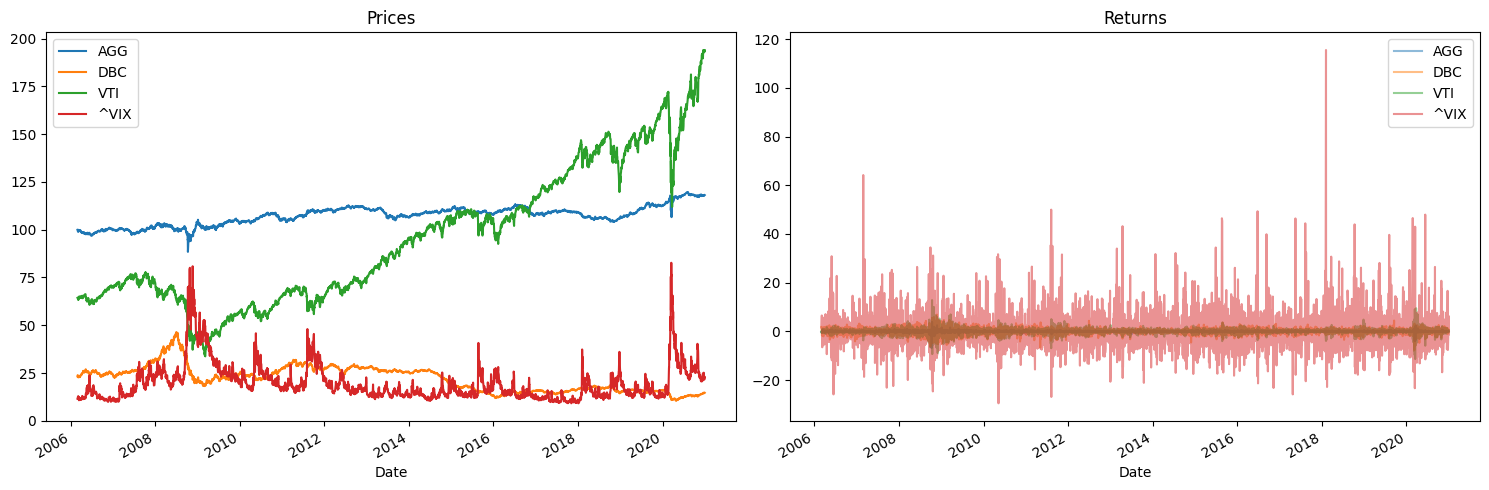
\includegraphics[width=0.8
    \linewidth]{images/prices_returns_assets.png}
    \caption{Prices and returns of VIX, AGG, DBC and VTI from 2006 to 2020}
    \label{fig:enter-label}
\end{figure}

\subsection{Synthetic Gaussian Data}
\label{subsec:synthetic_results}

We simulate four time series using a multivariate normal distribution with parameters $\Sigma$ and $\mu$ estimated from the previously described assets.

The Markowitz approach is implemented using a rolling window of 500 days. At each step, we compute the optimal portfolio weights using $\hat{\Sigma}$ and $\hat{\mu}$ from the last 500 days, solving the quadratic programming problem detailed before.

For the sequential neural networks (RNN, LSTM, GRU), models are adapted to output four neurons per hidden layer. These models are trained to directly maximize the Sharpe ratio over a fixed 250-day window, with the loss function computed as the average Sharpe ratio over this period. Each model undergoes a 4-year (1,000 observations) training phase before any portfolio weights are computed. Testing is conducted over 2 years (504 observations), followed by retraining using the test data.

This methodology allows for a direct comparison of portfolio allocations derived from the Markowitz model and the neural networks.

Figure \ref{fig:synthetic_allocations} illustrates the allocation trajectories for the Markowitz model and the neural networks under synthetic returns. 

1. \textbf{Weights convergence for both models:}  
The weights converge for both models, requiring fewer rolling window days for the neural network (250 days vs. 500 days for the Markowitz model).

2. \textbf{Remarks on results:}  
As mentioned the optimal solution can be determined using a quadratic program with the true parameters $\Sigma$ (covariance matrix) and $\mu$ of the data generation process. In this specific context, the Markowitz Portfolio is optimal and it's approximation is really close to the optimal solution.



\subsection{Real Data with Non-Gaussian Dynamics}

We apply the same optimization framework used for synthetic data to real-world data. After several checks (volatility clustering, leverage effects, and Gaussianity tests in the annexes), it is clear that we are far from a Gaussian setting. Real returns exhibit heavy tails, volatility clustering, and complex temporal dependencies that violate the core assumptions of Markowitz.

\paragraph{Allocation Results.}
The results show that the portfolio weights learned by neural models adapt much more frequently at each time step compared to Markowitz. This dynamic adjustment allows the neural models to better capture changing market conditions. Additionally, the cumulative returns demonstrate higher gains for most neural models, with the GRU specifically outperforming the others. The RNN, with its more chaotic weight adjustments, struggles as expected due to its inability to capture long-term dependencies between assets, preventing it from outperforming LSTM and GRU.

As for Markowitz, it performs the worst, with weights that are likely poorly estimated due to non-Gaussianity and its inability to detect nonlinear dependencies between assets. This highlights the limitations of traditional mean-variance optimization in real-world, non-Gaussian markets.




\begin{figure}[!h]
    \centering
    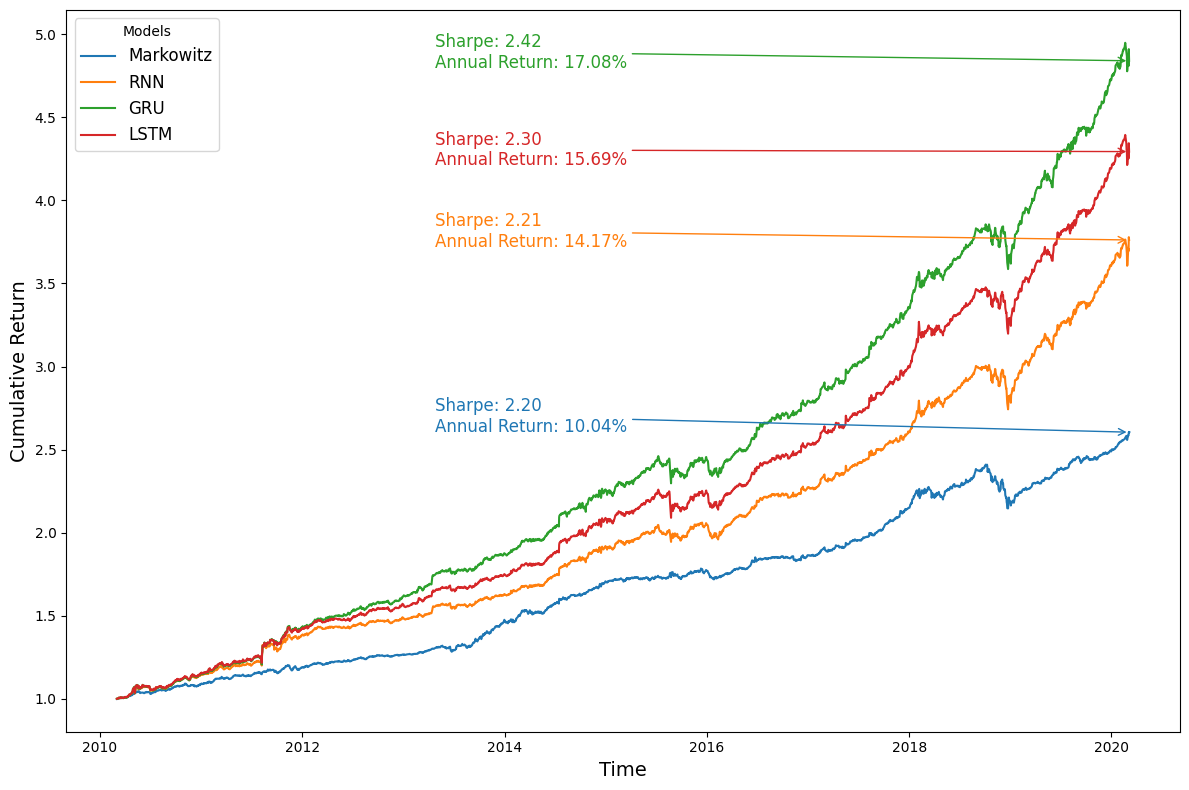
\includegraphics[width=0.6\textwidth]{images/cumreturn_real.png}
    \caption{Cumulative returns on real data: Markowitz vs.\ neural approaches. The neural models can benefit from learning temporal patterns that deviate from Gaussian assumptions.}
    \label{fig:realdata_performance}
\end{figure}

\subsection{Conclusion of Empirical Findings}
Our rolling experiments on both synthetic and real data lead to two main conclusions:
\begin{itemize}
    \item \textbf{Synthetic (Gaussian) Scenario:} Markowitz and sequential neural networks converge to the same allocation, reaffirming that mean--variance optimization is optimal under normality.
    \item \textbf{Real (Non-Gaussian) Scenario:} The neural models—especially LSTM and GRU—exhibit can slightly outperform Markowitz. We can infer that the models can learn some temporal features such as leverage effects, volatility clusters, and higher-order moments. However, the well known problem of these neural networks is the lack of interpretation for the model's outputs.
\end{itemize}
Consequently, while Markowitz remains a robust baseline for controlled settings, our results show that deep sequential networks provide valuable flexibility in more realistic, non-Gaussian markets.





\section{Conclusion}
On synthetic data drawn from a true multivariate Gaussian, Markowitz and sequential neural networks converge to essentially the same optimal portfolio. However, real financial returns often exhibit heavier tails, volatility clustering, and time-varying correlations that violate Markowitz's core assumptions. In such settings, we find that neural networks---by directly modeling temporal dependencies---can attain improved Sharpe ratios, but with higher variations.

\vspace{10pt}
\noindent
\textbf{Future Work.} During the project, we did not conduct a comprehensive ablation study to precisely assess the empirical impact of certain hyperparameters. This analysis could be the focus of future work to further optimize the potential performance of sequential neural networks for our specific task. Further penalization for additional transaction costs arising from frequent re-balancing of the portfolio weights should also be studied in further details.   


\clearpage

\printbibliography

\clearpage

\section*{Annexes}

\begin{figure}
    \centering
    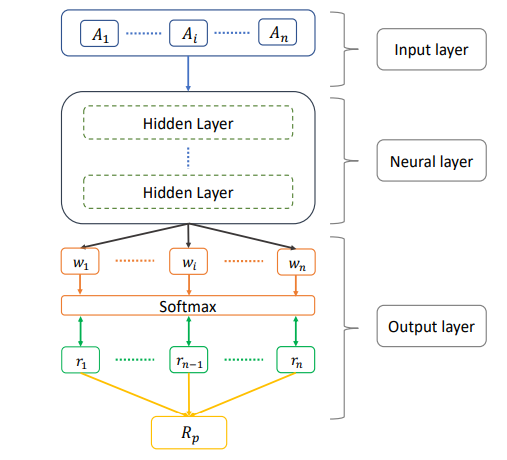
\includegraphics[width=0.5\linewidth]{images/architecture_model.PNG}
    \caption{Overall model's architecture}
    \label{fig:enter-label}
\end{figure}

The $A_i$ values represent the past returns. The neural network layer produces weights $w_1, \dots, w_n$, which are subsequently normalized using a softmax layer with a temperature parameter $T$. These normalized weights are then used to compute the Sharpe ratio of the portfolio. The hyperparameters and the implementation can be found in the Github repo.

\clearpage

\label{subsec:realdata_results}


\begin{figure}[h]
    \centering

    \begin{subfigure}[b]{0.45\textwidth}
        \centering
        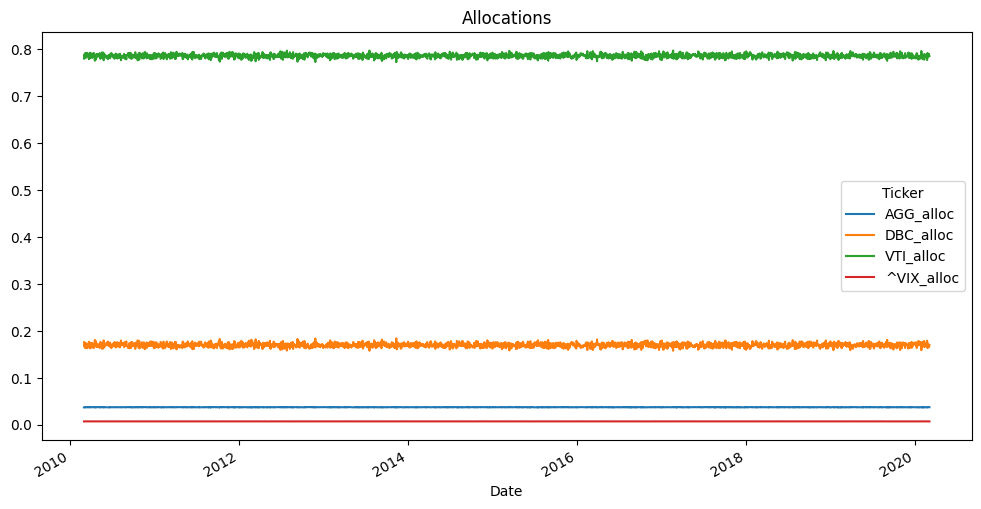
\includegraphics[width=\textwidth]{images/allocations_rnn_synthetic.png}
        \caption{RNN}
    \end{subfigure}
    \hfill
    \begin{subfigure}[b]{0.45\textwidth}
        \centering
        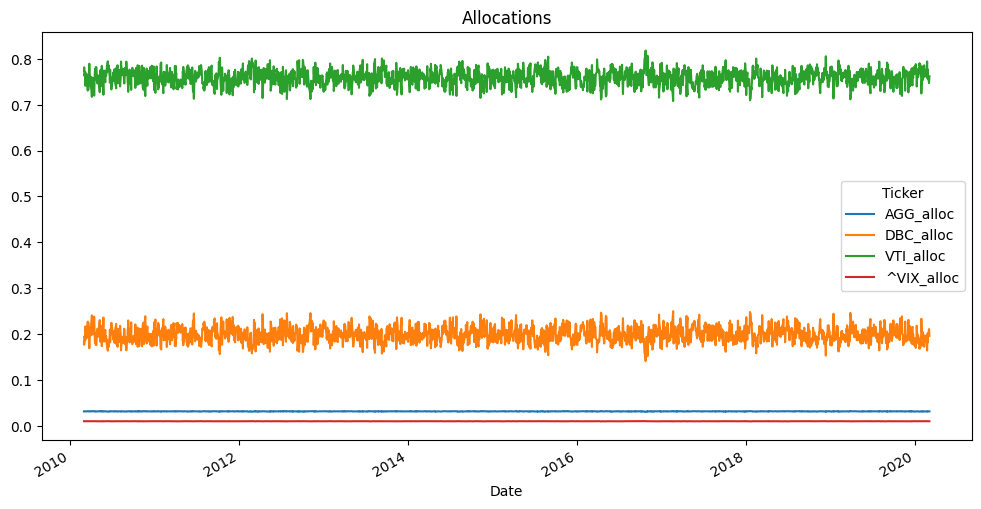
\includegraphics[width=\textwidth]{images/allocations_lstm_synthetic.png}
        \caption{LSTM}
    \end{subfigure}

    \vskip\baselineskip 
    \begin{subfigure}[b]{0.45\textwidth}
        \centering
        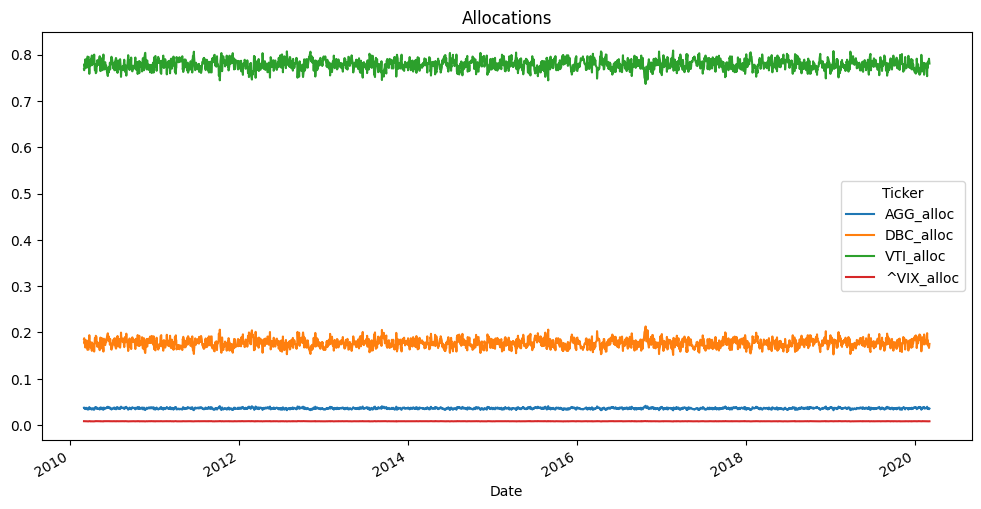
\includegraphics[width=\textwidth]{images/allocations_gru_synthetic.png}
        \caption{GRU}
    \end{subfigure}
    \hfill
    \begin{subfigure}[b]{0.45\textwidth}
        \centering
        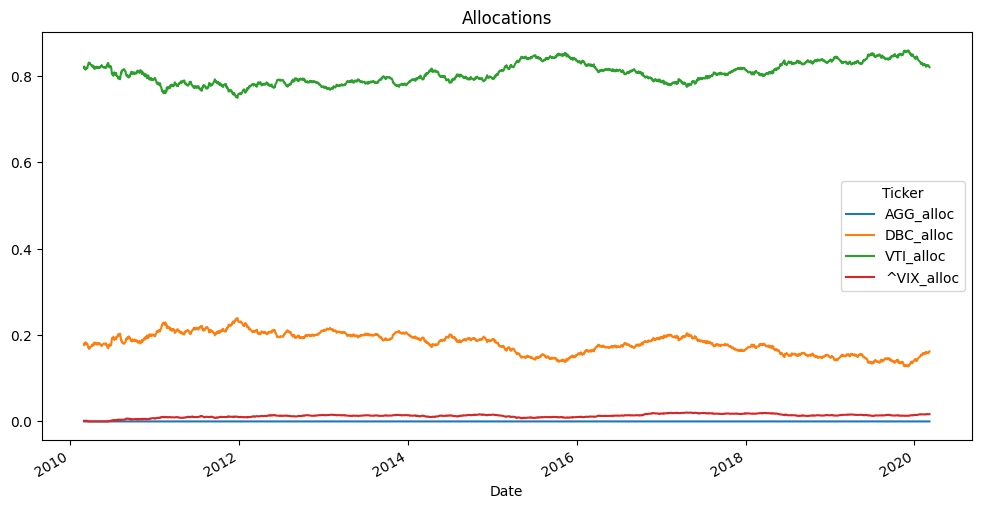
\includegraphics[width=\textwidth]{images/allocations_markow_synthetic.png}
        \caption{Markowitz}
    \end{subfigure}
    \caption{Allocation paths on synthetic Gaussian data. All sequential models converge to the same weights as the Markowitz solver. }
    \label{fig:synthetic_allocations}
\end{figure}



\begin{figure}[h]
    \centering

    \begin{subfigure}[b]{0.45\textwidth}
        \centering
        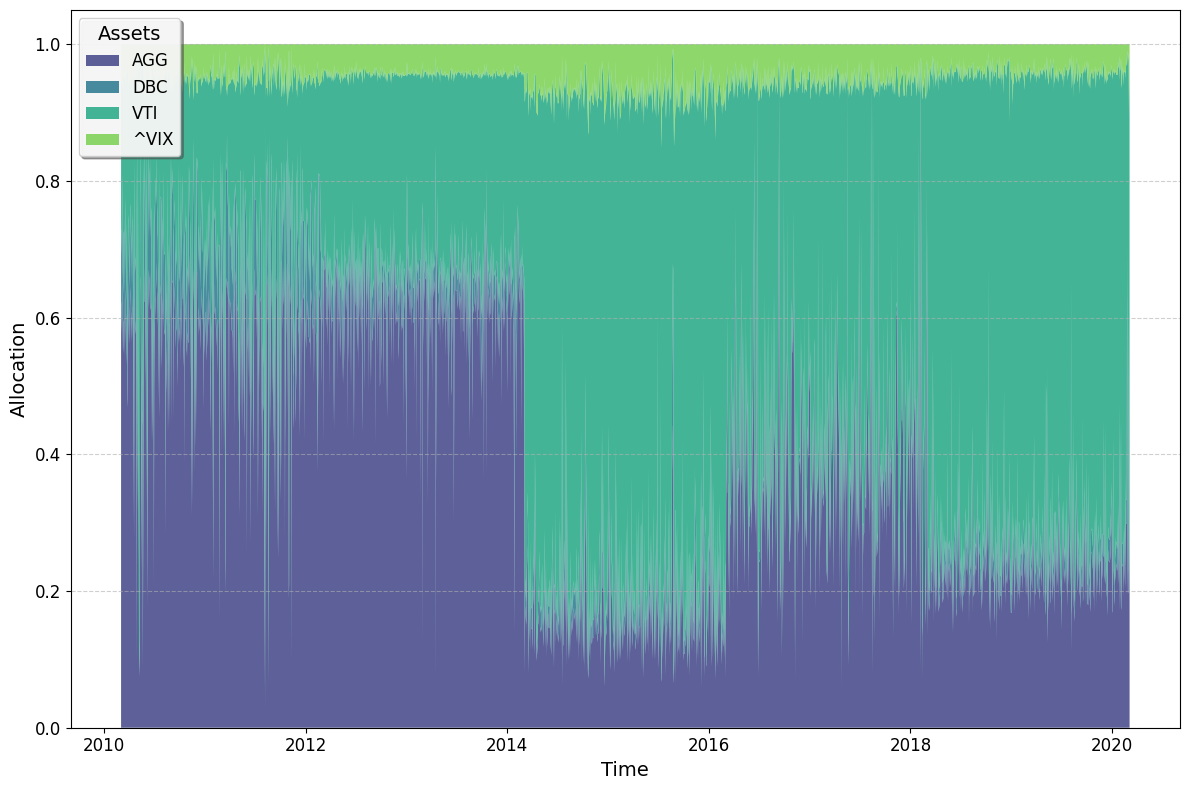
\includegraphics[width=\textwidth]{images/stackplot_rnn.png}
        \caption{RNN}
    \end{subfigure}
    \hfill
    \begin{subfigure}[b]{0.45\textwidth}
        \centering
        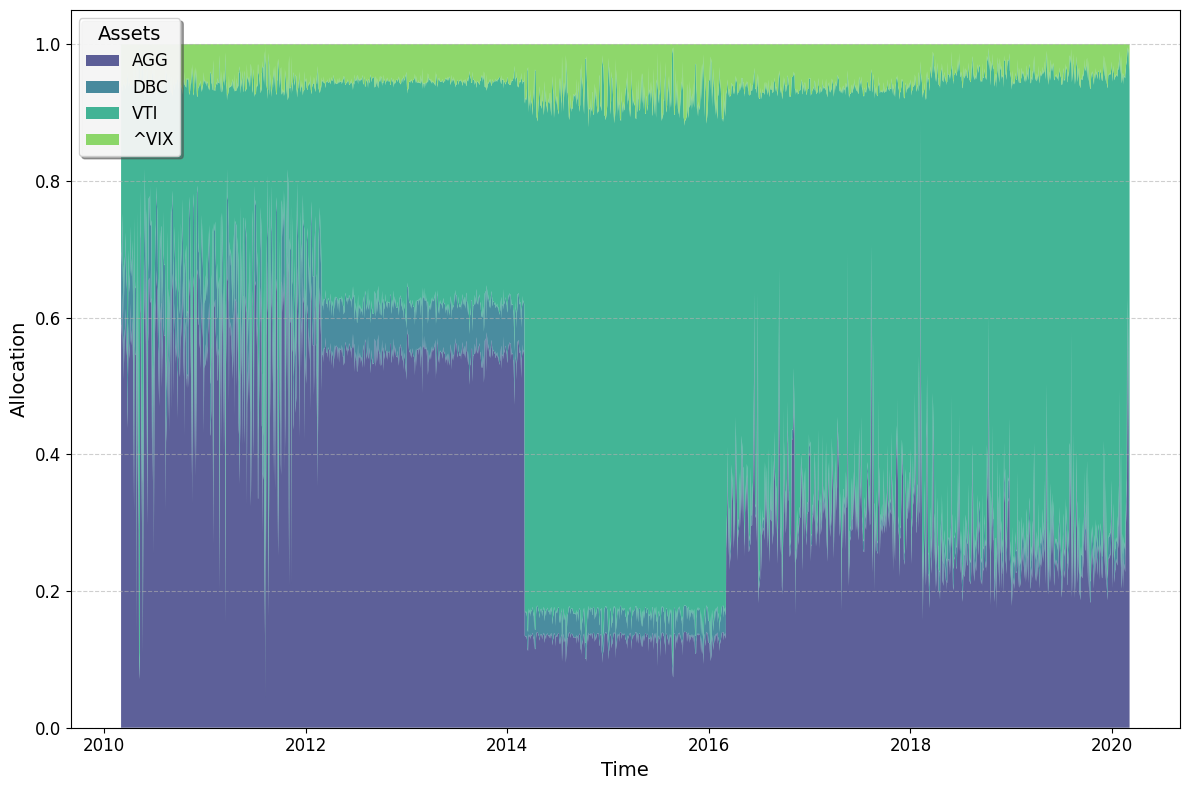
\includegraphics[width=\textwidth]{images/stackplot_lstm.png}
        \caption{LSTM}
    \end{subfigure}

    \vskip\baselineskip 
    \begin{subfigure}[b]{0.45\textwidth}
        \centering
        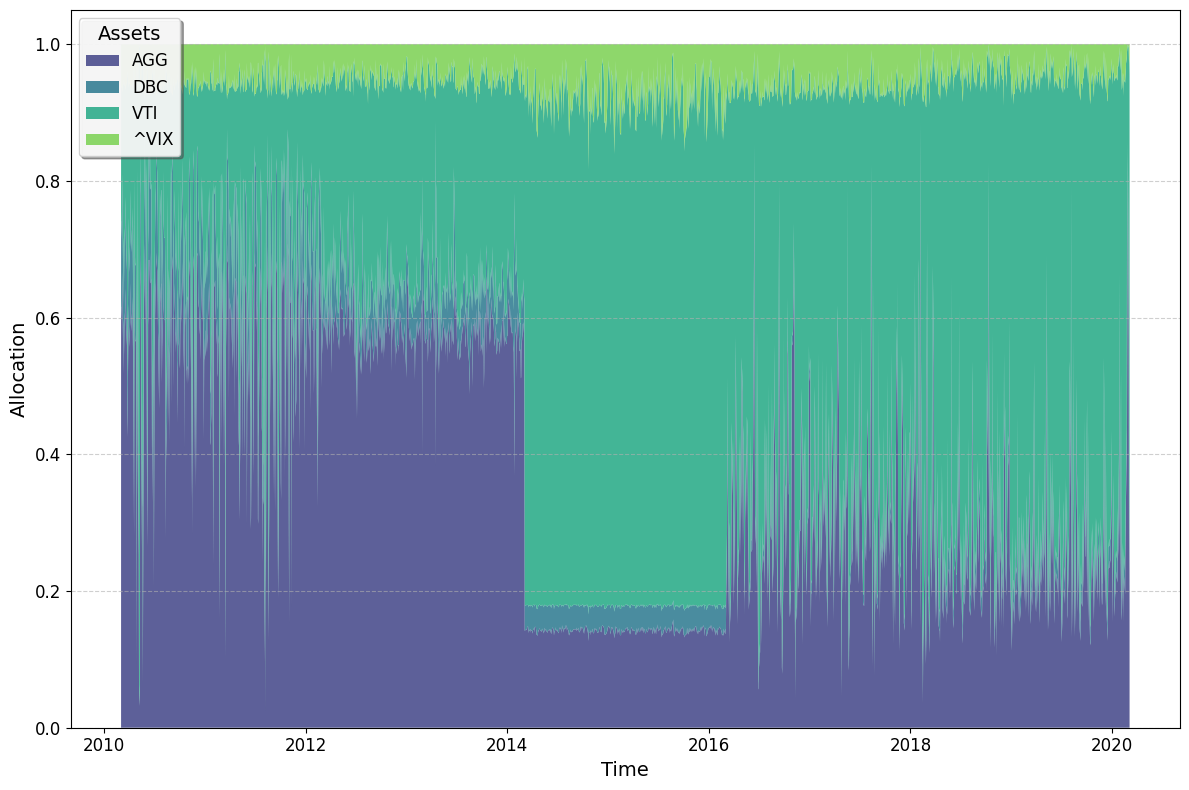
\includegraphics[width=\textwidth]{images/stackplot_gru.png}
        \caption{GRU}
    \end{subfigure}
    \hfill
    \begin{subfigure}[b]{0.45\textwidth}
        \centering
        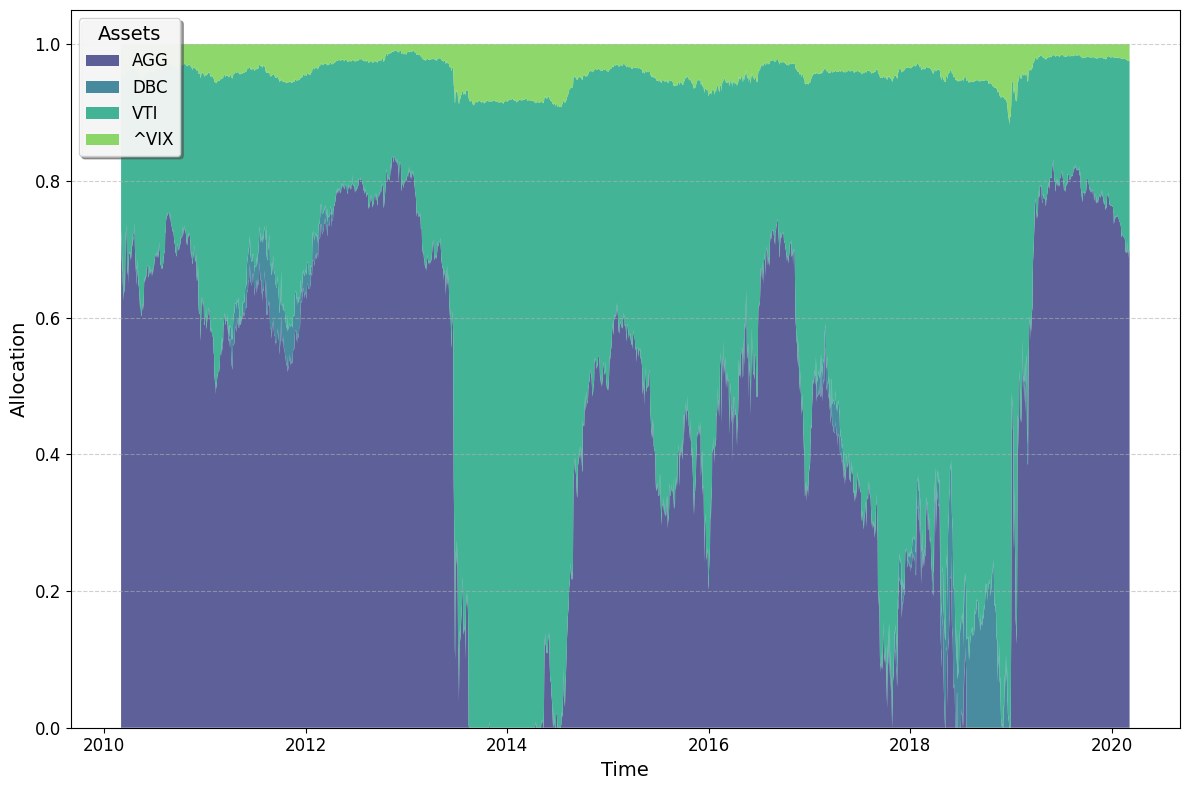
\includegraphics[width=\textwidth]{images/stackplot_marko.png}
        \caption{Markowitz}
    \end{subfigure}
    \caption{Assets allocations of the models on real assets. Note that we do not penalize for transaction costs, this would likely smooth the obtained weights by decreasing the frequency of rebalancing.}
    \label{fig:realdata_allocations}
\end{figure}

\clearpage

\begin{figure}[!h]
    \centering
    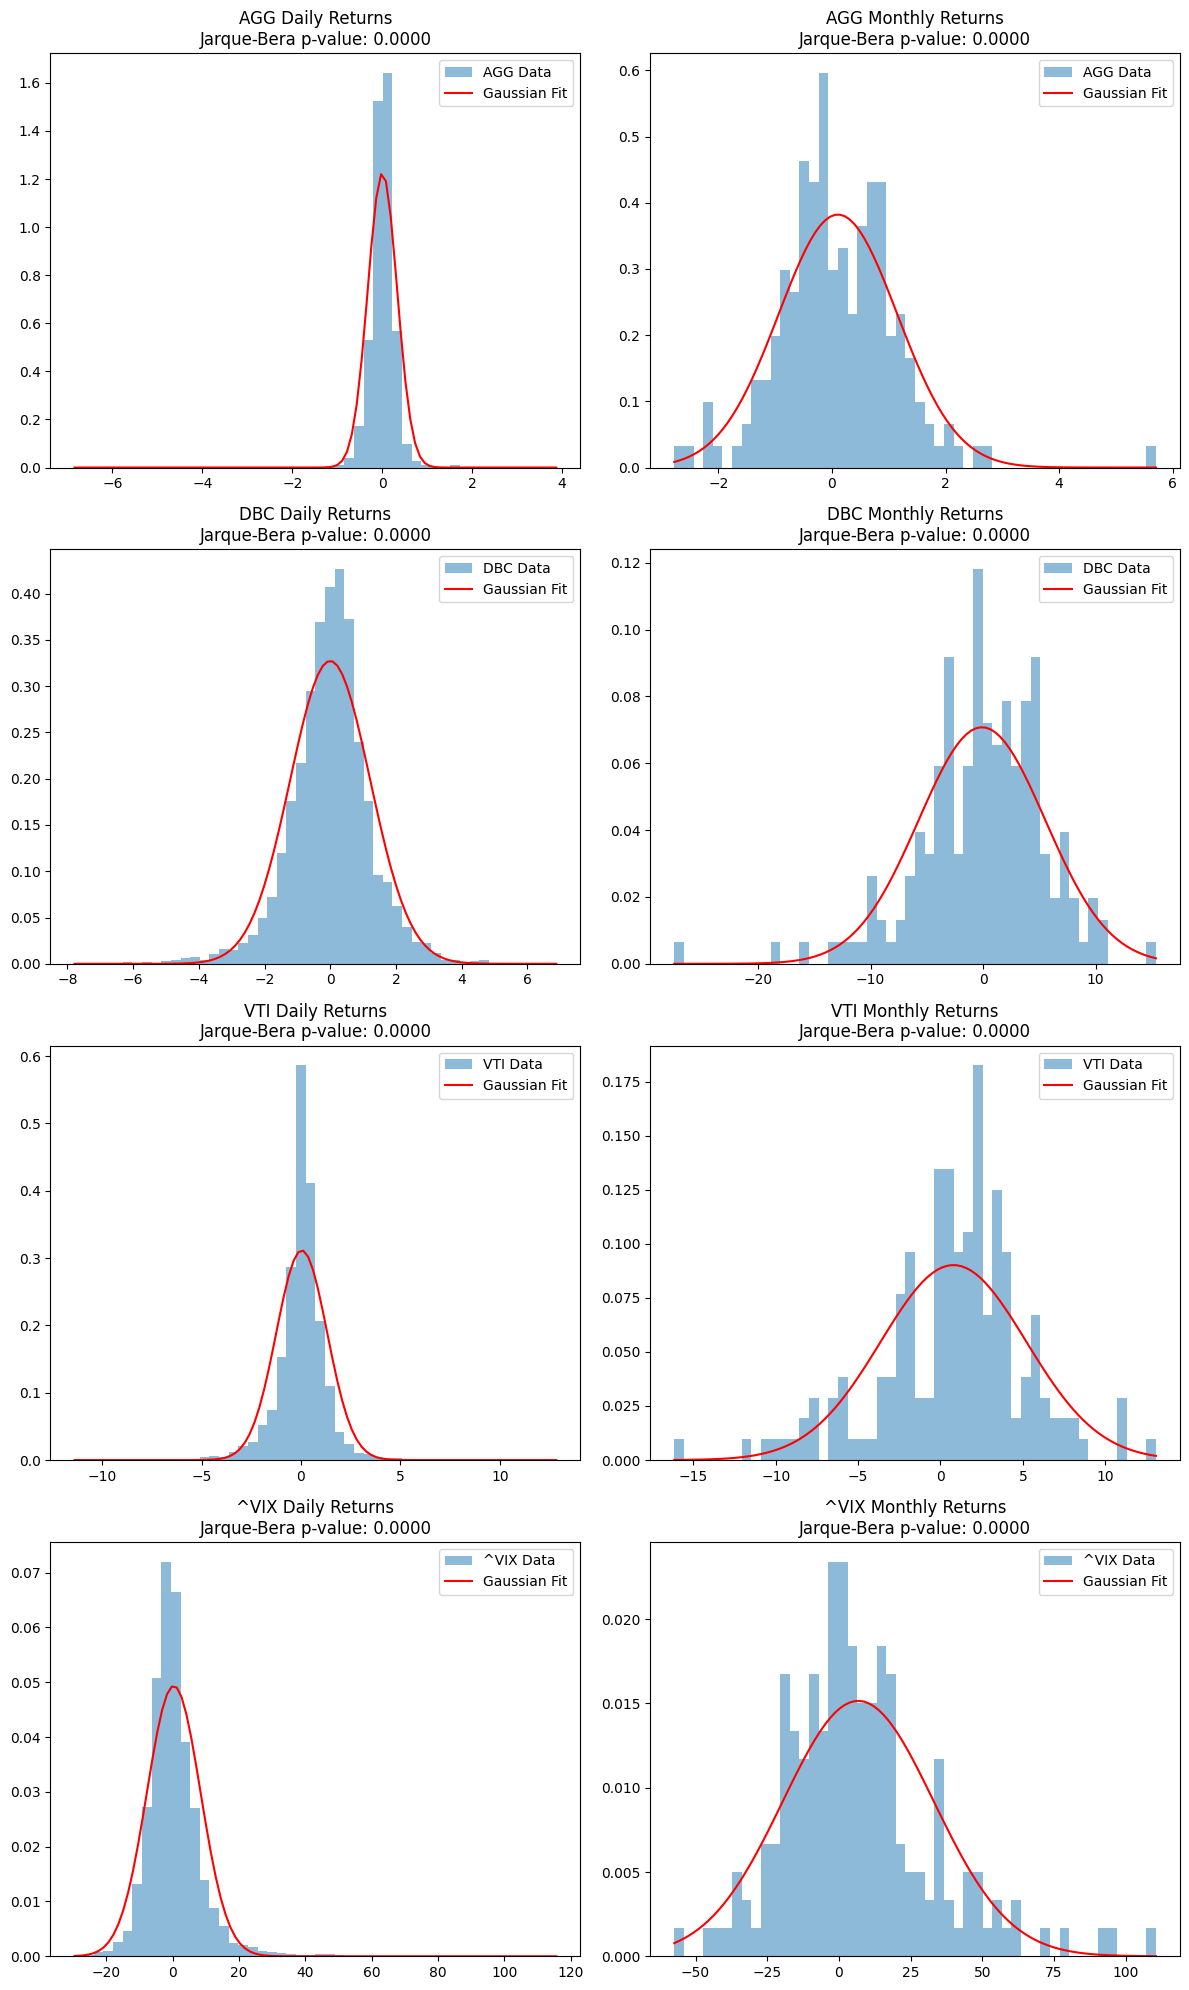
\includegraphics[width=0.45\textwidth]{images/real_data_distribution.png}
    \caption{Empirical distributions of daily/monthly returns (histograms) vs.\ fitted normal distributions (solid lines). We observe that real returns have heavier tails and mild skewness.}
    \label{fig:realdata_distributions}
\end{figure}


\begin{figure}
    \centering
    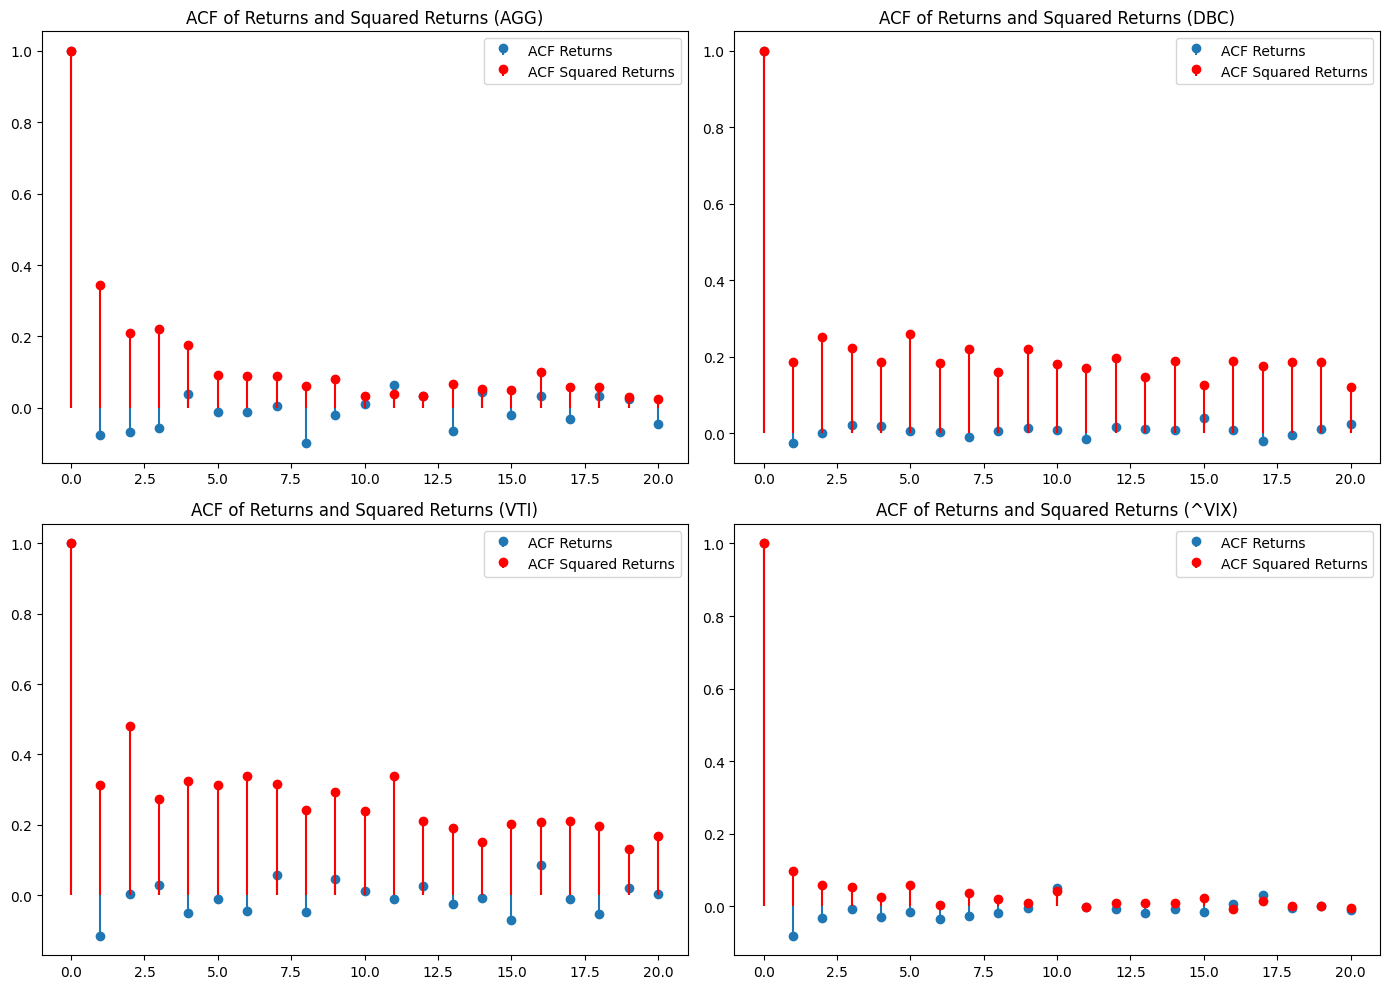
\includegraphics[width=0.5\linewidth]{images/acf_real.png}
    \caption{Auto Correlation Function of the returns and the squared returns. We observed an alignment with well documented stylized facts  on financial time series : absence of memory of returns (almost no autocorrelation for simple returns) while significant autocorrelation of squared returns that reflects conditional volatility as well as volatility clustering ie persistence of observed ACF of squared returns.}
    \label{fig:enter-label}
\end{figure}

\clearpage

\begin{figure}
    \centering
    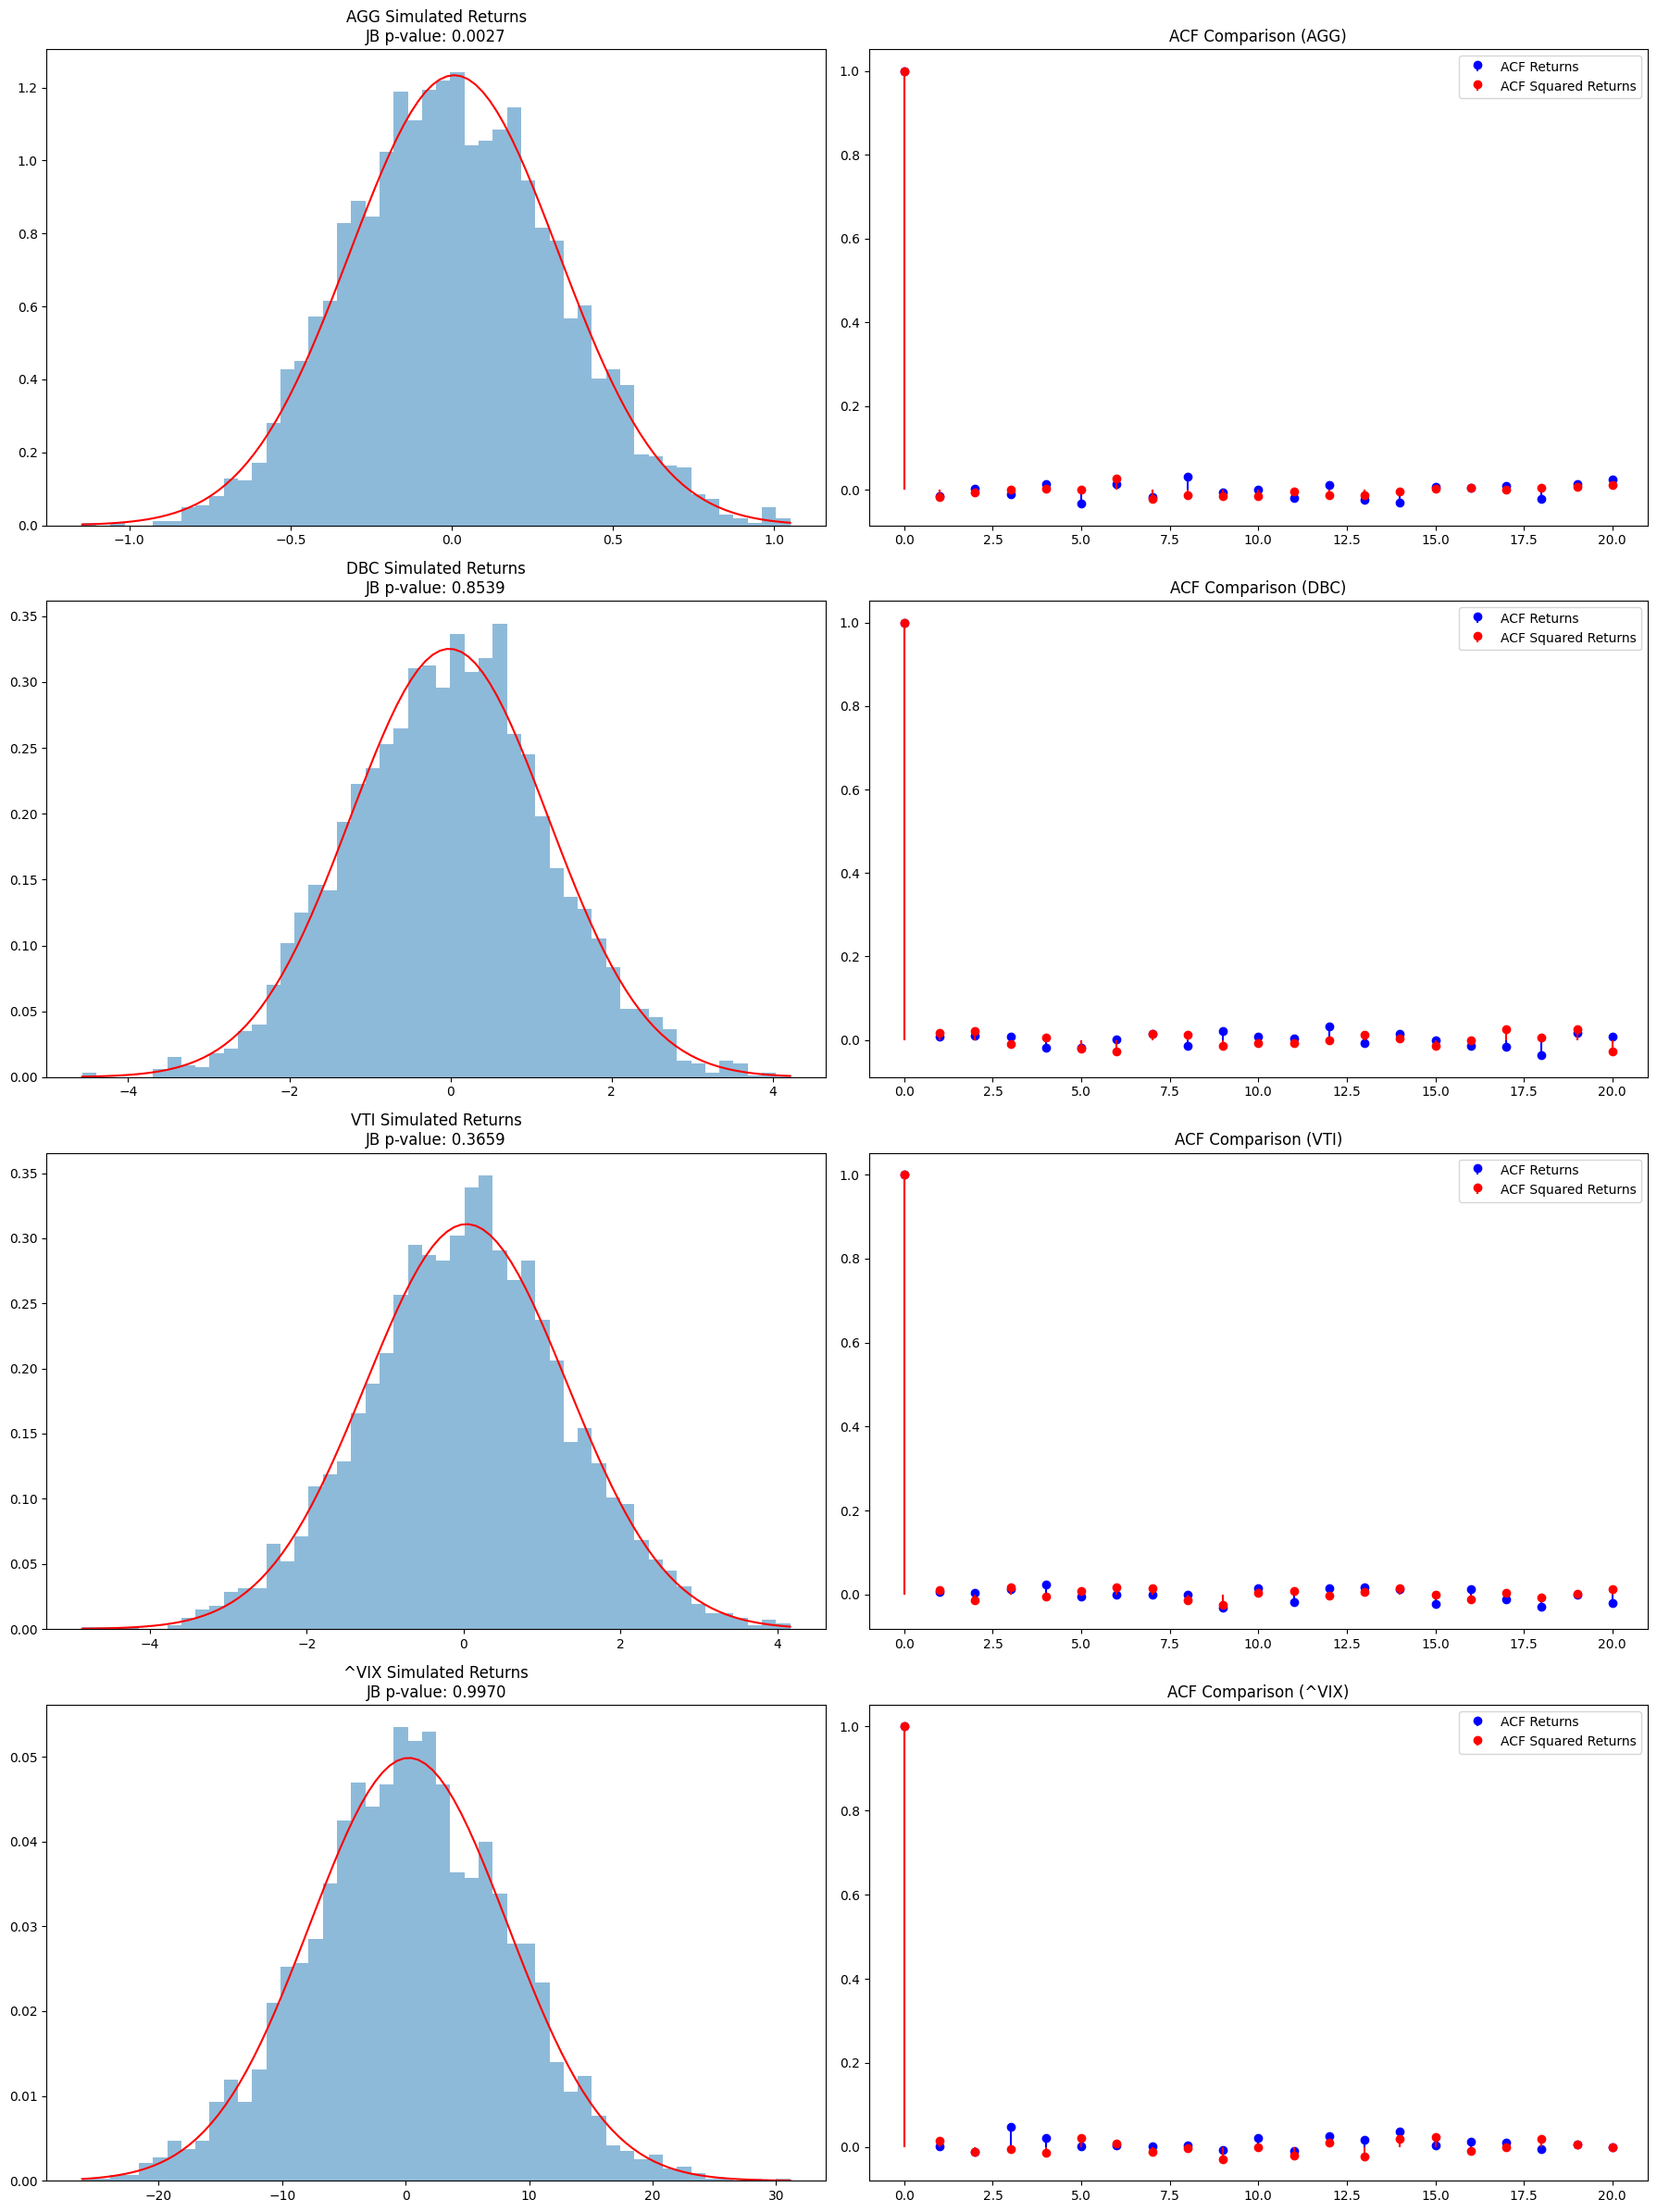
\includegraphics[width=0.5\linewidth]{images/multivariate_gaussian_estimated_distrib_acf.png}
    \caption{As a comparison we display the same plots than figure 6 and 7 for simulated gaussian data, this highlights the inability of naive gaussian simulation to capture important empirical properties of asset returns.}
    \label{fig:enter-label}
\end{figure}

\clearpage

\underline{Leverage Effect}  
 

The \textit{leverage effect} is a well-known stylized fact on financial time series. It states that there is a negative correlation between past returns and future asset volatilities. Specifically, volatility tends to increase when returns are lower than expected and decrease when returns exceed expectations. This empirical phenomenon, identified by Bouchaud, has been observed in both stock indices and individual stocks.


\begin{figure}
    \centering
    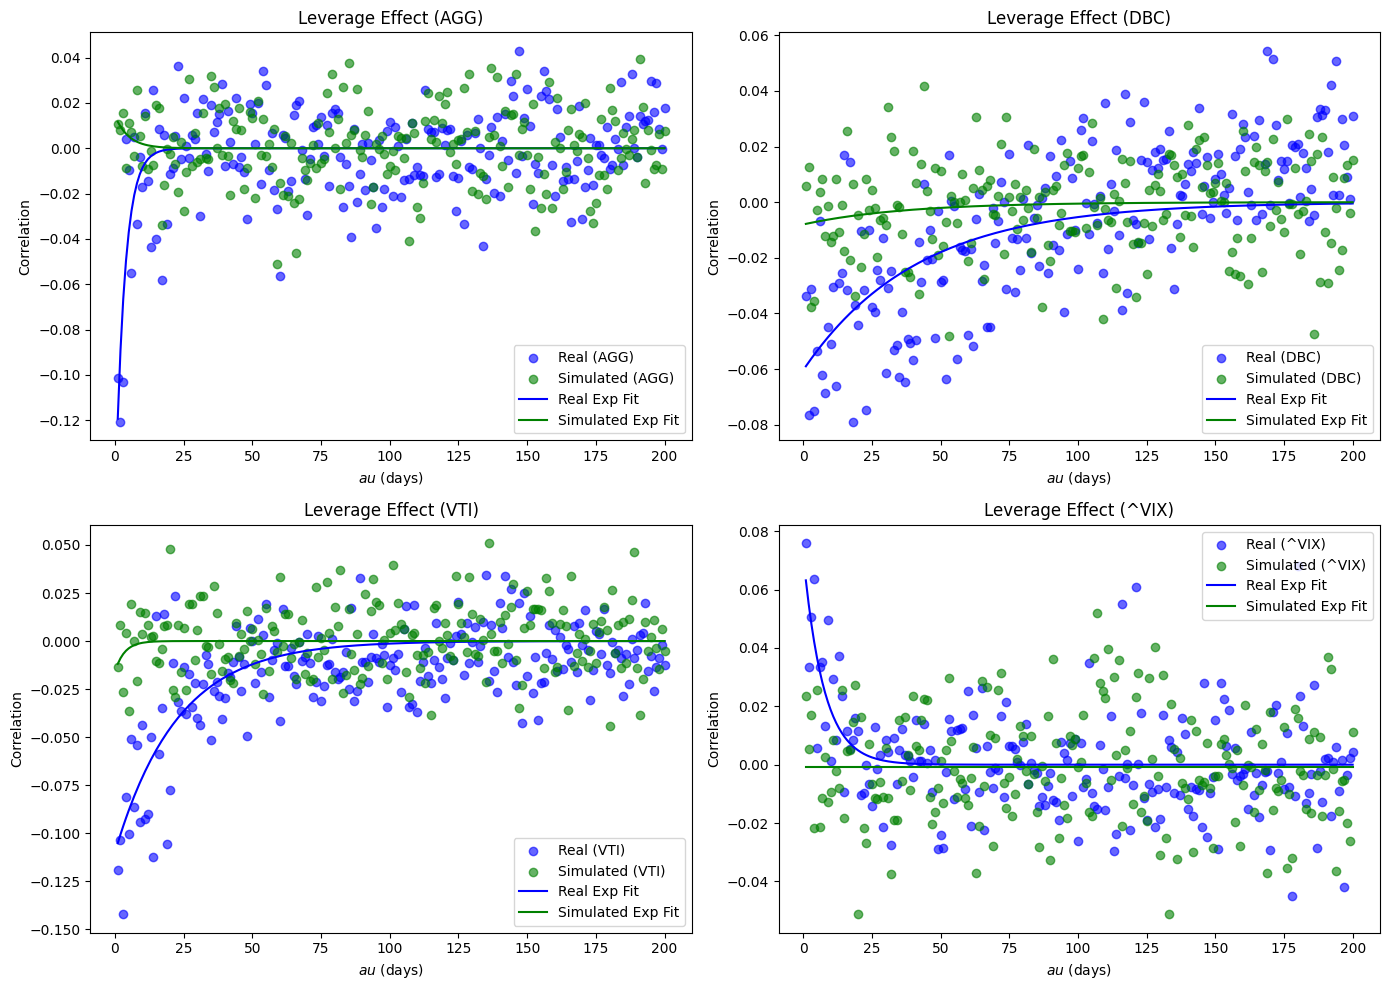
\includegraphics[width=1\linewidth]{images/leverage_effect.png}
    \caption{Estimating \textit{leverage effect} on both synthetic and real assets.}
    \label{fig:enter-label}
\end{figure}


\end{document}
